\documentclass[11pt,a4paper]{article}

\usepackage[T1]{fontenc}
\usepackage[utf8]{inputenc}
\usepackage{charter}
\usepackage[a4paper,margin=2.4cm]{geometry}
\usepackage{microtype}
\usepackage{amsmath}
\usepackage{booktabs}
\usepackage{tabularx}
\usepackage{graphicx}
\usepackage{xcolor}
\usepackage{caption}
\usepackage{enumitem}
\usepackage{tikz}
\usetikzlibrary{positioning,arrows.meta,calc}
\usepackage[numbers,sort&compress]{natbib}
\usepackage[colorlinks=true,linkcolor=black,citecolor=black,urlcolor=blue!60!black]{hyperref}

\captionsetup{font=small,labelfont=bf,margin=0.5cm}
\setlist{itemsep=2pt,topsep=4pt}
\newcommand{\code}[1]{\texttt{\small #1}}
% \input that works inside tabular (plain TeX primitive)
\makeatletter\newcommand{\tabinput}[1]{\@@input #1 }\makeatother
\definecolor{c1}{HTML}{2a78d6}
\definecolor{c2}{HTML}{eb6834}
\definecolor{c3}{HTML}{1baf7a}
\definecolor{c4}{HTML}{eda100}

\title{\textbf{Evaluating Hallucination Detectors for RAG Systems}}
\author{Shakhzodbek Bakhtiyorov\\\small\href{mailto:shakhzodbek.bakhtiyorov@gmail.com}{shakhzodbek.bakhtiyorov@gmail.com}}
\date{September 2026}

\begin{document}
\maketitle

\begin{abstract}
\noindent
Detecting answers that are not supported by the retrieved context is a prerequisite
for monitoring retrieval-augmented generation (RAG) systems. We compare four
faithfulness detectors on HaluBench while holding the judge model fixed
(\code{gpt-4o-mini}), so that differences reflect the evaluation protocol rather than
model capability: a holistic LLM judge, a claim-level LLM judge (LLM-Claims), G-Eval,
and LLM claim extraction followed by natural language inference (NLI). On a stratified
sample of 1{,}198 examples from six subsets, the three
LLM-based detectors are statistically indistinguishable (accuracy 79.6--82.2\%,
ROC-AUC 83.9--84.9\%), while the NLI pipeline is far weaker (accuracy 59.2\%) because
it labels correct paraphrases as unsupported. On RAGTruth, the only subset with
naturally occurring hallucinations, LLM-Claims ranked hallucinations best but its
decision rule missed them. In a pre-registered follow-up on 700 held-out RAGTruth
answers, flagging an answer when \emph{any} claim fails raised recall from 36.3\% for
the holistic judge's verdict to 76.6\% at similar precision (50.0\% vs.\ 48.4\%); even
with its threshold tuned post hoc, the holistic judge reached at most 46.8\% recall at
50\% precision. All three pre-registered hypotheses were supported with paired bootstrap
confidence intervals excluding zero. These findings are limited to one dataset of
natural hallucinations (124 positive examples) and one judge model.
\end{abstract}

% =====================================================================
\section{Introduction}

A RAG system can retrieve the right passage and still generate an answer that adds or
alters facts. Because human review of every answer is not feasible in production,
automatic faithfulness detection is needed to monitor such systems.

Using a large language model as a judge is now the common approach, but a single model
can serve as a judge in several ways: it can be asked for one verdict on the whole
answer~\citep{ravi2024lynx}, asked to judge each atomic claim separately, following the
decomposition idea of FActScore~\citep{min2023factscore}, or asked for a graded score
on a rubric~\citep{liu2023geval}. Cheaper non-LLM alternatives based on natural
language inference are also used, for example in RAGAS~\citep{es2024ragas}. Published
comparisons usually change the model and the protocol at the same time, which makes it
hard to tell how much the protocol itself matters.

This report holds the judge model fixed and addresses three research questions:
\begin{enumerate}[label=\textbf{RQ\arabic*.}, leftmargin=*]
  \item With the same model, do holistic, claim-level and rubric-based judging differ
        in how well they detect hallucinations?
  \item How does a claim-extraction + NLI pipeline compare with LLM judges?
  \item Does the answer depend on the kind of hallucination: synthetic perturbations
        versus hallucinations that occur naturally in RAG outputs?
\end{enumerate}

\paragraph{Contributions.}
(i) A controlled comparison of four detectors on six HaluBench subsets, with bootstrap
confidence intervals and paired tests; (ii) an analysis of why NLI-based checking fails
on RAG answers; (iii) a pre-registered, held-out test showing that on RAGTruth's
naturally occurring hallucinations a claim-level judge with an ``any failing claim''
rule substantially improves recall at similar precision; and (iv) an open, resumable evaluation harness with 29
offline tests.

% =====================================================================
\section{Detectors}
\label{sec:detectors}

All four detectors receive the same (question, document, answer) triple. Each returns
a binary decision (hallucinated or not) and a continuous hallucination score in
$[0,1]$, so both thresholded and threshold-free metrics can be computed.
Figure~\ref{fig:protocols} summarises the protocols and Table~\ref{tab:detectors} their
details.

\begin{figure}[t]
\centering
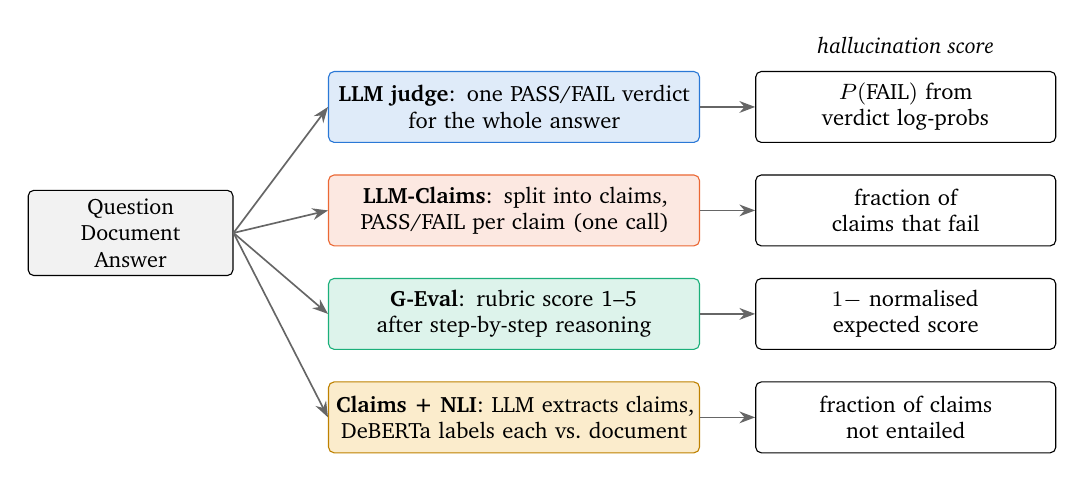
\begin{tikzpicture}[
  node distance=4mm and 7mm,
  box/.style={draw, rounded corners=2pt, align=center, font=\footnotesize,
              minimum height=9mm, inner sep=3pt},
  arr/.style={-{Stealth[length=2mm]}, semithick, draw=black!60}]
  \node[box, fill=black!5, minimum width=26mm] (in) {Question\\Document\\Answer};
  \node[box, right=12mm of in, yshift=16mm, fill=c1!15, draw=c1, text width=45mm] (j)
       {\textbf{LLM judge}: one PASS/FAIL verdict\\for the whole answer};
  \node[box, below=of j, fill=c2!15, draw=c2, text width=45mm] (c)
       {\textbf{LLM-Claims}: split into claims,\\PASS/FAIL per claim (one call)};
  \node[box, below=of c, fill=c3!15, draw=c3, text width=45mm] (g)
       {\textbf{G-Eval}: rubric score 1--5\\after step-by-step reasoning};
  \node[box, below=of g, fill=c4!20, draw=c4!80!black, text width=45mm] (n)
       {\textbf{Claims + NLI}: LLM extracts claims,\\DeBERTa labels each vs.\ document};
  \node[box, right=of j, text width=36mm] (sj) {$P(\text{FAIL})$ from\\verdict log-probs};
  \node[box, right=of c, text width=36mm] (sc) {fraction of\\claims that fail};
  \node[box, right=of g, text width=36mm] (sg) {$1-$ normalised\\expected score};
  \node[box, right=of n, text width=36mm] (sn) {fraction of claims\\not entailed};
  \foreach \t in {j,c,g,n} \draw[arr] (in.east) -- (\t.west);
  \draw[arr] (j) -- (sj); \draw[arr] (c) -- (sc); \draw[arr] (g) -- (sg); \draw[arr] (n) -- (sn);
  \node[font=\footnotesize\itshape, above=1mm of sj] {hallucination score};
\end{tikzpicture}
\caption{The four evaluation protocols. All LLM steps use \code{gpt-4o-mini} at
temperature~0, so the protocols differ only in how the question is posed and how the
output becomes a score.}
\label{fig:protocols}
\end{figure}

\begin{table}[t]
\centering\small
\caption{Detector details. Decision rules were fixed before any evaluation and were not
tuned on the data.}
\label{tab:detectors}
\begin{tabularx}{\textwidth}{@{}l X l l@{}}
\toprule
Detector & Decision rule (main run) & Calls / answer & Based on \\
\midrule
LLM judge    & The model's own PASS/FAIL verdict & 1 & HaluBench / Lynx prompt \citep{ravi2024lynx} \\
LLM-Claims   & Hallucinated if $>50\%$ of claims fail & 1 & Claim decomposition \citep{min2023factscore} \\
G-Eval       & Hallucinated if score $>0.5$ & 1 & \citet{liu2023geval} \\
Claims + NLI & Any contradiction, or $>60\%$ of claims neutral & 1 + local model & e.g.\ RAGAS \citep{es2024ragas} \\
\bottomrule
\end{tabularx}
\end{table}

For the NLI detector, the cross-encoder \code{cross-encoder/nli-deberta-v3-large}
accepts roughly 512 tokens. Documents are therefore split into overlapping 400-token
windows, each paired with the claim as a proper (premise, hypothesis) pair; a claim
counts as entailed if any window entails it. This avoids truncating the claim itself
when the document is long.

% =====================================================================
\section{Experimental setup}
\label{sec:setup}

\paragraph{Data.}
HaluBench~\citep{ravi2024lynx} contains about 15{,}000 (question, document, answer)
triples from six sources, each labelled PASS (faithful) or FAIL (hallucinated). In
five subsets the hallucinated answers are constructed: generated by an LLM (HaluEval) or
perturbed from correct answers (FinanceBench, DROP, CovidQA, PubMedQA). In RAGTruth
they are real outputs of RAG systems annotated by humans (Table~\ref{tab:data}).

\begin{table}[t]
\centering\small
\caption{Evaluation data. The main run draws 200 examples per subset; the held-out run
uses every RAGTruth example not used in the main run.}
\label{tab:data}
\setlength{\tabcolsep}{4pt}
\begin{tabular}{@{}l l l r r@{}}
\toprule
Subset & Domain & Hallucinated answers & Main: $n$ (FAIL) & Held-out: $n$ (FAIL) \\
\midrule
HaluEval     & General QA                 & LLM-generated         & 200 (100) & -- \\
RAGTruth     & Mixed RAG tasks            & Natural, human-labelled & 200 (36) & 700 (124) \\
FinanceBench & Financial filings          & Perturbed             & 200 (100) & -- \\
DROP         & Wikipedia, numerical       & Perturbed             & 200 (100) & -- \\
CovidQA      & COVID-19 research papers   & Perturbed             & 200 (100) & -- \\
PubMedQA     & Biomedical abstracts       & Perturbed             & 200 (100) & -- \\
\bottomrule
\end{tabular}
\end{table}

\paragraph{Sampling.}
Examples are drawn with a fixed seed and stratified by label, keeping each subset's own
label ratio. This matters because HaluBench is ordered by label: taking the first $N$
rows, as an earlier version of this project did, returns a single class for several
subsets and makes precision, recall and F1 meaningless.

\paragraph{Metrics.}
The positive class is ``hallucinated''. We report accuracy, balanced accuracy,
precision, recall and F1 for binary decisions, and ROC-AUC and PR-AUC for continuous
scores. RAGTruth is imbalanced (18\% hallucinated), so always answering ``faithful''
already reaches 82\% accuracy; balanced accuracy, F1 and PR-AUC are the informative
metrics there.

\paragraph{Statistics.}
95\% confidence intervals are percentile bootstrap intervals over examples (1{,}000
resamples in the main run, 2{,}000 in the held-out run). Differences between detectors
use a paired bootstrap on the same examples; a difference is considered established only
when its interval excludes zero.

\paragraph{Error handling.}
A failed API call or unparseable reply is recorded as an error, never as ``faithful''.
Two of 1{,}200 main-run examples still failed after retries (one unparseable
LLM-Claims reply, one failed claim extraction for NLI); they are excluded for every
detector so that all detectors are compared on the same examples. The held-out run had
no errors.

% =====================================================================
\section{Results on HaluBench}
\label{sec:results}

\subsection{Overall comparison}

Table~\ref{tab:overall} shows that the three LLM-based detectors perform almost
identically, while claims + NLI is 23 accuracy points behind (RQ1, RQ2).

\begin{table}[t]
\centering\footnotesize
\setlength{\tabcolsep}{3.5pt}
\caption{Pooled results on 1{,}198 HaluBench examples (\%,
95\% bootstrap CI). $\Delta$ is the paired difference in accuracy to the LLM judge.
Cost is API cost per 1{,}000 answers at \$0.15/\$0.60 per million input/output tokens.}
\label{tab:overall}
\begin{tabular}{@{}l c c c c c c r@{}}
\toprule
Detector & Accuracy & Bal.\ acc. & F1 & ROC-AUC & PR-AUC & $\Delta$ accuracy & USD \\
\midrule
\tabinput{tables/overall.tex}
\bottomrule
\end{tabular}

\smallskip
\raggedright\footnotesize\textsuperscript{a}\,Plus local inference of the NLI model
(about 3 hours for 1{,}200 answers on Apple silicon).
\end{table}

The ROC-AUCs of the three LLM detectors (83.9--84.9) have overlapping intervals.
LLM-Claims' accuracy gap to the judge is not distinguishable from zero. G-Eval is
slightly less accurate, but its interval only just excludes zero and it is one of three
comparisons, so this is weak evidence. With \code{gpt-4o-mini}, neither claim
decomposition nor log-probability weighting improves on a single holistic verdict
across HaluBench as a whole.

For context, the holistic judge's macro-averaged accuracy (82.2\%) lies in the range
reported by \citet{ravi2024lynx} for Lynx-8B (82.9\%) and Llama-3-70B (80.1\%), below
GPT-4o (86.5\%) and above RAGAS faithfulness (66.9\%). Their figures cover the full
benchmark and other models, so this comparison is indicative only.

\subsection{Per-subset results}

\begin{figure}[t]
\centering
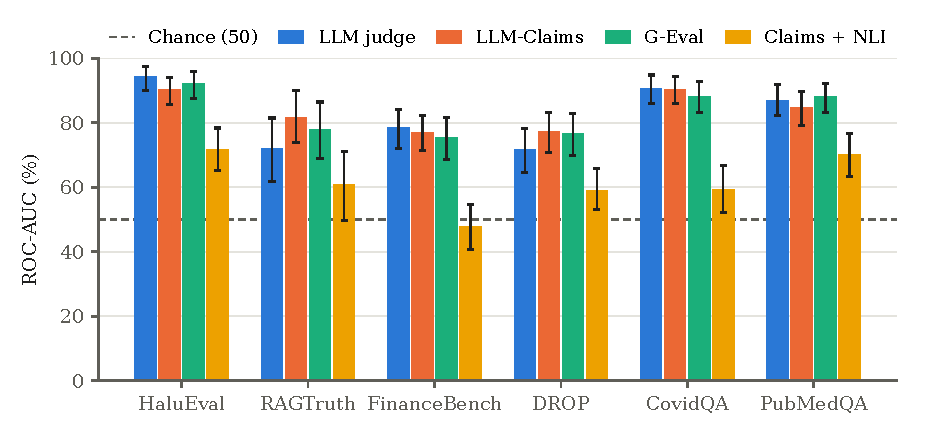
\includegraphics[width=\textwidth]{figures/roc_auc_by_subset.pdf}
\caption{ROC-AUC per HaluBench subset with 95\% bootstrap intervals (200 examples per
subset; 199 for HaluEval and FinanceBench after error exclusion). The three LLM
detectors are close on every subset; NLI is near chance on FinanceBench.}
\label{fig:subsets}
\end{figure}

Figure~\ref{fig:subsets} shows that the LLM detectors track each other closely on most
subsets. The exceptions are RAGTruth and DROP, where LLM-Claims ranks hallucinations
better than the holistic judge (81.8 vs.\ 72.1 and 77.4 vs.\ 71.7), although per-subset
intervals overlap at this sample size. HaluEval is the only subset where the holistic
judge leads on accuracy (92.5\% vs.\ 85.9\% for LLM-Claims), with barely overlapping
intervals.

\subsection{Why NLI fails}

Claims + NLI flags 47\% of faithful answers as hallucinated (312 of 663) and still
misses 33\% of hallucinations (178 of 536). Of the 312 false alarms, 195 stem from
correct claims labelled \emph{neutral}: the NLI model does not treat paraphrases,
summaries, or claims that combine two sentences as entailed. The remaining 117 stem
from spurious \emph{contradiction} labels. On FinanceBench, where answers depend on
numbers from tables, its ROC-AUC (47.7) is at chance.

An earlier version of this pipeline reported 76\% accuracy for NLI. That figure was an
artifact of the sampling problem described in Section~\ref{sec:setup}: on subsets where
every sampled answer was hallucinated, a detector that over-flags appears accurate.

\subsection{A pattern on RAGTruth}
\label{sec:pattern}

On RAGTruth, accuracy is uninformative: all LLM detectors score 81--83\%, the same as
always answering ``faithful''. LLM-Claims had the best ranking (ROC-AUC 81.8) but the
worst F1 (14.6), because its rule ``more than 50\% of claims fail'' let almost every
hallucination through. Only 3 of the 36 hallucinated answers crossed 50\%, whereas 27
of 36 had at least one failing claim (compared with 25 of 164 faithful answers).

This suggests that natural hallucinations are usually a minority of wrong claims inside
otherwise correct answers. Because the pattern was found on the evaluation data itself,
it was treated as a hypothesis and tested on new data.

% =====================================================================
\section{Pre-registered held-out test on RAGTruth}
\label{sec:holdout}

\subsection{Design}

Before any held-out example was scored, the following hypotheses, decision rules, data
and analysis were written down (\code{docs/ragtruth\_holdout.md} in the repository):
\begin{itemize}[leftmargin=*]
  \item \textbf{H1} (replication, threshold-free): LLM-Claims ranks hallucinations
        better than the holistic judge (ROC-AUC).
  \item \textbf{H2} (decision rule): ``any claim fails'' outperforms ``more than 50\% of
        claims fail'' (F1).
  \item \textbf{H3} (practical): LLM-Claims with the ``any'' rule outperforms the
        holistic judge (F1).
\end{itemize}
The held-out set comprises every RAGTruth example not used in the main run: 700
answers, 124 hallucinated. Detectors, prompts and model are unchanged; only the
LLM-Claims threshold differs, and both rules are computed from the same saved scores. A
hypothesis is supported if the 95\% paired bootstrap interval of the difference
excludes zero in the stated direction.

\subsection{Results}

\begin{figure}[t]
\centering
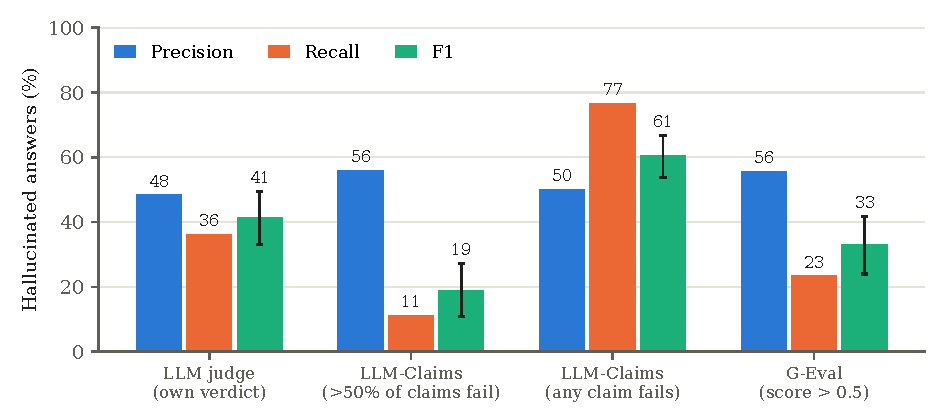
\includegraphics[width=\textwidth]{figures/holdout_rules.pdf}
\caption{Precision, recall and F1 per decision rule on 700 held-out RAGTruth answers
(124 hallucinated). Whiskers on F1 show 95\% bootstrap intervals. Flagging an answer
when any claim fails roughly doubles recall relative to the judge's own verdict, at
similar precision.}
\label{fig:rules}
\end{figure}

\begin{table}[t]
\centering\footnotesize
\setlength{\tabcolsep}{3pt}
\caption{Held-out RAGTruth results (\%, 95\% bootstrap CI; $n=700$, 124 hallucinated).
The two LLM-Claims rows share one set of scores, so their ROC-AUC and PR-AUC are
identical by construction. Accuracy is omitted: every rule scores 82--83\%, the same as
always answering ``faithful''.}
\label{tab:holdout}
\begin{tabular}{@{}l c c c c c c@{}}
\toprule
Decision rule & Prec. & Recall & F1 & Bal.\ acc. & ROC-AUC & PR-AUC \\
\midrule
\tabinput{tables/holdout.tex}
\bottomrule
\end{tabular}
\end{table}

\begin{figure}[t]
\centering
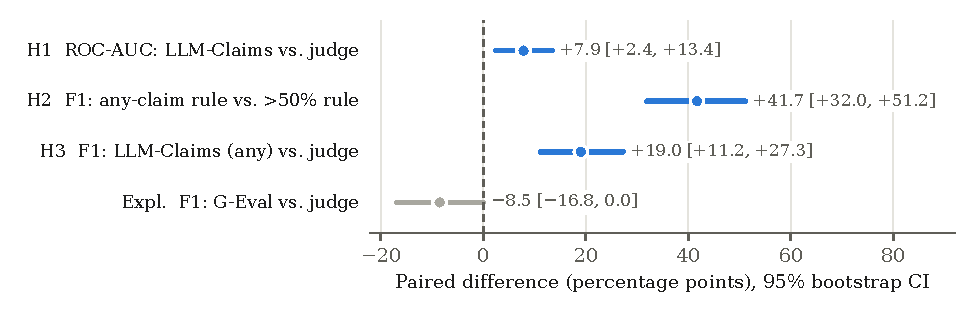
\includegraphics[width=\textwidth]{figures/holdout_forest.pdf}
\caption{Paired differences for the pre-registered hypotheses (blue) and one exploratory
comparison (grey), in percentage points with 95\% bootstrap intervals (2{,}000
resamples). All three pre-registered intervals exclude zero.}
\label{fig:forest}
\end{figure}

\begin{table}[t]
\centering\small
\caption{Hypothesis tests on the held-out set (paired bootstrap, percentage points).}
\label{tab:hypotheses}
\begin{tabular}{@{}l l r c l@{}}
\toprule
& Comparison & $\Delta$ & 95\% CI & Outcome \\
\midrule
\tabinput{tables/hypotheses.tex}
\bottomrule
\end{tabular}
\end{table}

As Figure~\ref{fig:rules} and Table~\ref{tab:holdout} show, the holistic judge catches
36\% of hallucinated answers, whereas LLM-Claims with the ``any'' rule catches 77\%.
Both are correct about half the time when they raise a flag (precision 48\% and 50\%).
The original ``more than 50\%'' rule is the most precise but misses 89\% of
hallucinations.

All three hypotheses are supported (Figure~\ref{fig:forest},
Table~\ref{tab:hypotheses}). Balanced accuracy, a secondary outcome, agrees with H3
($+16.1$ points, CI $[11.4, 20.8]$). The G-Eval comparison was exploratory; its interval
touches zero.

\subsection{Is the comparison fair to the judge?}

Recall at a single operating point favours whichever detector has the better-chosen
threshold. The judge also outputs a continuous score, $P(\text{FAIL})$, so a lower
cut-off could buy it more recall. In an exploratory analysis (not pre-registered) we
therefore swept the judge's threshold over all observed values on the held-out set. Its
scores are almost binary (the median is 0.0 and the 90th percentile 1.0), so lowering the
cut-off helps little: at precision $\geq 50\%$ its best recall is 46.8\%, and at
precision $\geq 45\%$ it is 55.6\%. These are best cases, tuned on the test data itself;
LLM-Claims with its pre-declared rule reaches 76.6\% recall at 50.0\% precision. The
advantage is therefore not an artifact of the judge's default threshold, but its size is
closer to $1.6\times$ than $2\times$ against a tuned judge. The threshold-free comparison
(H1, ROC-AUC $+7.9$ points) is the fairest single summary.

\subsection{Consistency with the development sample}

The held-out estimates closely reproduce the numbers first observed on the 200 main-run
RAGTruth answers: F1 with the ``any'' rule 61.4 $\rightarrow$ 60.5, LLM-Claims ROC-AUC
81.8 $\rightarrow$ 81.1, and the judge's ROC-AUC 72.1 $\rightarrow$ 73.2. The detectors
behave consistently on new data, and the effect is not an artifact of one sample.

% =====================================================================
\section{Discussion}
\label{sec:discussion}

In our experiments the evaluation protocol mattered little on the synthetic subsets and
substantially on RAGTruth, the one subset with natural hallucinations (RQ3). Whether
this holds for natural hallucinations in general needs more datasets to establish.

\paragraph{Synthetic subsets.}
In five subsets the hallucinated answer is a deliberate perturbation of a correct one: a
changed number, a swapped entity, an added unsupported statement. A likely explanation
for the tie is that the error is then prominent, so a holistic verdict and a
claim-by-claim check detect the same thing.

\paragraph{Natural hallucinations.}
Natural hallucinations appear to be mostly one or a few unsupported details inside an
otherwise correct, often long answer. Asked for one overall verdict, the judge weighs many correct
statements against one wrong one and often answers PASS; asked about each claim
separately, it has to rule on the wrong detail on its own. The per-claim scores are
consistent with this (Section~\ref{sec:pattern}).

\paragraph{The decision rule is part of the method.}
The same LLM-Claims scores yield an F1 of 18.8 or 60.5 depending only on the threshold.
Ranking ability (ROC-AUC) and usefulness at a fixed cut-off can diverge sharply, which
is why both are reported and why the rule was fixed before the held-out test.

\paragraph{NLI is not a cheap substitute.}
Off-the-shelf NLI cross-encoders are trained on short, literal premise--hypothesis
pairs, whereas RAG answers paraphrase and summarise. The pipeline is cheaper in API cost
but loses 23 accuracy points, which makes it unsuitable as a standalone detector here.

\paragraph{Practical recommendations.}
\begin{itemize}[leftmargin=*]
  \item To monitor a RAG system, use a claim-level LLM judge and flag an answer when
        any claim fails. It costs about $1.9\times$ a holistic judge (\$0.32 vs.\ \$0.17
        per 1{,}000 answers on RAGTruth with \code{gpt-4o-mini}) and, in our RAGTruth
        experiments, catches substantially more hallucinations (76.6\% vs.\ 36.3\% for
        the judge's verdict, or at most 46.8\% with a tuned threshold). Validate this on
        your own data before relying on it.
  \item At 50\% precision, half of the flags are false alarms: use the detector to
        route answers to review, not to block them automatically.
  \item Evaluate detectors on naturally occurring hallucinations and report precision
        and recall rather than accuracy, which hides a detector that misses most
        hallucinations on imbalanced data.
  \item Keep the per-claim verdicts: they show which sentence failed, which speeds up
        review and error analysis.
\end{itemize}

% =====================================================================
\section{Limitations}
\label{sec:limitations}

\begin{itemize}[leftmargin=*]
  \item \textbf{One judge model.} All LLM steps used \code{gpt-4o-mini}. A stronger
        judge may catch single-claim errors in a holistic verdict and narrow the gap.
  \item \textbf{One prompt per detector.} LLM judges are sensitive to wording; the
        results hold for the prompts in the repository.
  \item \textbf{Generalisation of the main finding.} The claim-level advantage was shown
        on one dataset of natural hallucinations (RAGTruth, 124 positive examples in the
        held-out set), with one model and one prompt. It should be treated as a
        well-supported result for that setting, not as a general law for RAG systems.
  \item \textbf{Scope of the ``any'' rule.} It was tested only on RAGTruth; on the
        synthetic subsets it may raise more false alarms.
  \item \textbf{Sample size.} 200 examples per subset give per-subset intervals of
        roughly $\pm5$ accuracy points; only large per-subset differences are resolved.
  \item \textbf{Published baselines.} The Lynx figures cover the full benchmark and
        other models; they are context, not a head-to-head comparison.
  \item \textbf{Synthetic data.} Five of six subsets use constructed hallucinations,
        which may be easier to detect than those produced by deployed systems.
  \item \textbf{Pre-registration record.} The held-out hypotheses were written before
        the held-out run, but were not committed to version control beforehand, so no
        independent timestamp exists.
\end{itemize}

% =====================================================================
\section{Reproducibility}

All experiments run from the accompanying repository with one command each and cost
about \$1.60 in API calls in total (main run \$1.03, held-out run \$0.46). Sampling is
seeded and the exact example identifiers of each run are stored; LLM calls use
temperature~0, which is near-deterministic but not bit-identical across API versions.
Predictions are appended per example, so interrupted runs resume. The figures and
results tables in this report are generated directly from the saved result files by
\code{report/make\_figures.py}.

\begin{small}
\begin{verbatim}
python run_benchmark.py --out-dir results/main
python run_benchmark.py --subsets RAGTruth --n 0 --exclude-from results/main \
    --methods llm_judge llm_claims geval --claims-threshold 0 \
    --out-dir results/ragtruth_holdout
python run_benchmark.py --out-dir results/ragtruth_holdout --report-only \
    --bootstrap 2000
python report/make_figures.py
\end{verbatim}
\end{small}

% =====================================================================
\begin{thebibliography}{9}
\bibitem[Es et~al.(2024)]{es2024ragas}
S.~Es, J.~James, L.~Espinosa-Anke, and S.~Schockaert.
\newblock {RAGAS}: Automated evaluation of retrieval augmented generation.
\newblock In \emph{Proceedings of EACL 2024: System Demonstrations}, 2024.

\bibitem[Liu et~al.(2023)]{liu2023geval}
Y.~Liu, D.~Iter, Y.~Xu, S.~Wang, R.~Xu, and C.~Zhu.
\newblock {G-Eval}: {NLG} evaluation using {GPT-4} with better human alignment.
\newblock In \emph{Proceedings of EMNLP 2023}, 2023.

\bibitem[Min et~al.(2023)]{min2023factscore}
S.~Min, K.~Krishna, X.~Lyu, M.~Lewis, W.~Yih, P.~W. Koh, M.~Iyyer, L.~Zettlemoyer, and
H.~Hajishirzi.
\newblock {FActScore}: Fine-grained atomic evaluation of factual precision in long
form text generation.
\newblock In \emph{Proceedings of EMNLP 2023}, 2023.

\bibitem[Ravi et~al.(2024)]{ravi2024lynx}
S.~S. Ravi, B.~Mielczarek, A.~Kannappan, D.~Kiela, and R.~Qian.
\newblock Lynx: An open source hallucination evaluation model.
\newblock \emph{arXiv preprint arXiv:2407.08488}, 2024.
\newblock Dataset: \url{https://huggingface.co/datasets/PatronusAI/HaluBench}.
\end{thebibliography}

\end{document}
